\documentclass[10pt]{beamer}

% Package
\usepackage{graphicx}
\usepackage{tcolorbox}
\usepackage{listings}

% Theme
\usetheme{Warsaw}
\usecolortheme{beaver}

% Main & Info
\title[Angular]
{Module Angular}
\subtitle{Partie 3}
\author[Maxime Tournier]
{Maxime Tournier}
\date[21/08/2023]

% Start
\begin{document}

    \frame{\titlepage}

    \begin{frame}
        \frametitle{Sommaire}

        1. {Rappel} \newline
        2. {Back/Front} \newline
        3. {Json} \newline
        4. {HttpClient} \newline
        4. {Reprendre un projet} \newline
        5. {Build Angular} \newline
        6. {Déploiment Serveur} \newline

    \end{frame}

%%%%%%%% Présentation

    \begin{frame}
        \frametitle{Rappel}


        Créons un nouveau projet ensemble



    \end{frame}

%%%%%%%% Back/Front

    \begin{frame}
        \frametitle{Back/Front}

        Comprendre la fonctionnement du Back-Front

        \centering
        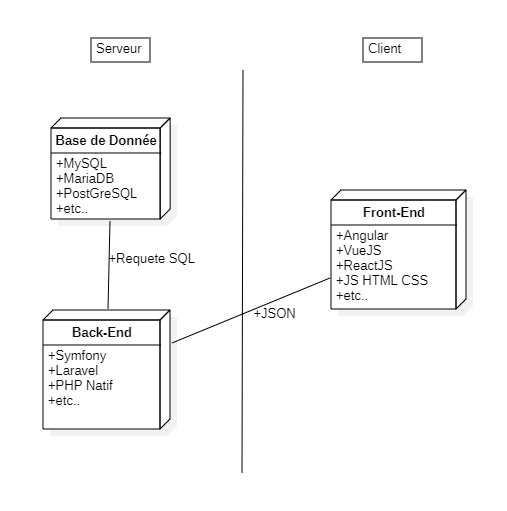
\includegraphics[width=9cm]{assets/backfront}

    \end{frame}

%%%%%%%% JSON

    \begin{frame}
        \frametitle{JSON}

        Le JavaScript Object Notation (JSON) \newline \newline

        Il s'agit d'un languague universel \newline \newline

        Il à pour but de changer d'interconnecter les donnée de tout les languague \newline \newline

        En concurance direct avec un autre langague XML \newline \newline



    \end{frame}

    \begin{frame}
        \frametitle{JSON}

        On utilise le JSON pour transmettre les donnée entre le back-end et le front-end \newline \newline

        Le Json peut servire a plein d'autre utilisation \newline \newline

        Objectif : Passé un object de L'API a angular grâce HttpClientModule \newline \newline

    \end{frame}

%%%%%%%% HttpClient

    \begin{frame}
        \frametitle{HttpClient}

        Comprendre et setup HttpClient

    \end{frame}

    \begin{frame}
        \frametitle{HttpClient}

        Ajouter HttpClientModule dans le module racine

    \end{frame}

    \begin{frame}
        \frametitle{HttpClient}

        Premier connexion grâve à l'API "https://api.chucknorris.io"

    \end{frame}

    \begin{frame}
        \frametitle{HttpClient}

        Activité Pokemon

    \end{frame}

    \begin{frame}
        \frametitle{HttpClient}

        Activité User

    \end{frame}

%%%%%%%% Reprendre un Projet

    \begin{frame}
        \frametitle{Reprendre un Projet}


    \end{frame}



%%%%%%%% Build Angular

    \begin{frame}
        \frametitle{Build Angular}


    \end{frame}


%%%%%%%% Déploiement Serveur

    \begin{frame}
        \frametitle{Déploiement Serveur}


    \end{frame}



\end{document}